
%% bare_jrnl.tex
%% V1.4b
%% 2015/08/26
%% by Michael Shell
%% see http://www.michaelshell.org/
%% for current contact information.
%%
%% This is a skeleton file demonstrating the use of IEEEtran.cls
%% (requires IEEEtran.cls version 1.8b or later) with an IEEE
%% journal paper.
%%
%% Support sites:
%% http://www.michaelshell.org/tex/ieeetran/
%% http://www.ctan.org/pkg/ieeetran
%% and
%% http://www.ieee.org/

%%*************************************************************************
%% Legal Notice:
%% This code is offered as-is without any warranty either expressed or
%% implied; without even the implied warranty of MERCHANTABILITY or
%% FITNESS FOR A PARTICULAR PURPOSE! 
%% User assumes all risk.
%% In no event shall the IEEE or any contributor to this code be liable for
%% any damages or losses, including, but not limited to, incidental,
%% consequential, or any other damages, resulting from the use or misuse
%% of any information contained here.
%%
%% All comments are the opinions of their respective authors and are not
%% necessarily endorsed by the IEEE.
%%
%% This work is distributed under the LaTeX Project Public License (LPPL)
%% ( http://www.latex-project.org/ ) version 1.3, and may be freely used,
%% distributed and modified. A copy of the LPPL, version 1.3, is included
%% in the base LaTeX documentation of all distributions of LaTeX released
%% 2003/12/01 or later.
%% Retain all contribution notices and credits.
%% ** Modified files should be clearly indicated as such, including  **
%% ** renaming them and changing author support contact information. **
%%*************************************************************************


% *** Authors should verify (and, if needed, correct) their LaTeX system  ***
% *** with the testflow diagnostic prior to trusting their LaTeX platform ***
% *** with production work. The IEEE's font choices and paper sizes can   ***
% *** trigger bugs that do not appear when using other class files.       ***                          ***
% The testflow support page is at:
% http://www.michaelshell.org/tex/testflow/



\documentclass[journal]{IEEEtran}

\ifCLASSOPTIONcompsoc
  % IEEE Computer Society needs nocompress option
  % requires cite.sty v4.0 or later (November 2003)
  \usepackage[nocompress]{cite}
\else
  % normal IEEE
  \usepackage{cite}
\fi



\usepackage{amsmath,graphicx,booktabs,amssymb}
%\usepackage{epstopdf}
\usepackage{epstopdf,algorithm2e}
\usepackage{multirow,caption}
\usepackage[export]{adjustbox}
\usepackage[pagebackref=false,breaklinks=true,colorlinks,bookmarks=false]{hyperref}

%\usepackage{algorithm}
\usepackage[noend]{algpseudocode}

\usepackage{subcaption}

\makeatletter
\def\BState{\State\hskip-\ALG@thistlm}
\makeatother

\usepackage{framed} 
\usepackage[framed]{ntheorem}

%\usepackage[pagebackref=true,breaklinks=true,colorlinks,bookmarks=false]{hyperref}
%\usepackage[pagebackref=false,breaklinks=true,colorlinks,bookmarks=false]{hyperref}
\graphicspath{{images/}{results/}}

\def\Fig#1{Fig.~\ref{fig:#1}}
\def\Eq#1{Eq.~(\ref{eq:#1})}
\def\Tab#1{Table~\ref{tab:#1}}
\def\Sec#1{Section~\ref{sec:#1}}
\def\Prop#1{Proposition~\ref{prop:#1}}

% A comment in a draft (shouldn't appear in the final version).
\newcommand{\comment}[2]{\( \P\){\bf #1: }{\rm \sf #2}\(\P\)}
% Comment this out in the draft
%\newcommand{\comment}[2]{}
\newcommand{\dbcomment}[1]{\comment{DB}{#1}}
\newcommand{\pgcomment}[1]{\comment{PG}{#1}}
\newcommand{\awcomment}[2]{\comment{AW}{#1}}
%---------------------------------

\def\eg{\emph{e.g.}, }
\def\Eg{\emph{E.g.}, }
\def\etal{\emph{et al.}}
\def\ie{\emph{i.e.}, }
\def\noi{\noindent}

%-----------------------
% Change the way IEEE write table caption
\usepackage{etoolbox}
\makeatletter
\patchcmd{\@makecaption}
  {\scshape}
  {}
  {}
  {}
\makeatletter
\patchcmd{\@makecaption}
  {\\}
  {.\ }
  {}
  {}
\makeatother
%\def\tablename{Table}
%-------------------------


\usepackage{listings}
%
% If IEEEtran.cls has not been installed into the LaTeX system files,
% manually specify the path to it like:
% \documentclass[journal]{../sty/IEEEtran}





% Some very useful LaTeX packages include:
% (uncomment the ones you want to load)


% *** MISC UTILITY PACKAGES ***
%
%\usepackage{ifpdf}
% Heiko Oberdiek's ifpdf.sty is very useful if you need conditional
% compilation based on whether the output is pdf or dvi.
% usage:
% \ifpdf
%   % pdf code
% \else
%   % dvi code
% \fi
% The latest version of ifpdf.sty can be obtained from:
% http://www.ctan.org/pkg/ifpdf
% Also, note that IEEEtran.cls V1.7 and later provides a builtin
% \ifCLASSINFOpdf conditional that works the same way.
% When switching from latex to pdflatex and vice-versa, the compiler may
% have to be run twice to clear warning/error messages.






% *** CITATION PACKAGES ***
%
%\usepackage{cite}
% cite.sty was written by Donald Arseneau
% V1.6 and later of IEEEtran pre-defines the format of the cite.sty package
% \cite{} output to follow that of the IEEE. Loading the cite package will
% result in citation numbers being automatically sorted and properly
% "compressed/ranged". e.g., [1], [9], [2], [7], [5], [6] without using
% cite.sty will become [1], [2], [5]--[7], [9] using cite.sty. cite.sty's
% \cite will automatically add leading space, if needed. Use cite.sty's
% noadjust option (cite.sty V3.8 and later) if you want to turn this off
% such as if a citation ever needs to be enclosed in parenthesis.
% cite.sty is already installed on most LaTeX systems. Be sure and use
% version 5.0 (2009-03-20) and later if using hyperref.sty.
% The latest version can be obtained at:
% http://www.ctan.org/pkg/cite
% The documentation is contained in the cite.sty file itself.






% *** GRAPHICS RELATED PACKAGES ***
%
\ifCLASSINFOpdf
  % \usepackage[pdftex]{graphicx}
  % declare the path(s) where your graphic files are
  % \graphicspath{{../pdf/}{../jpeg/}}
  % and their extensions so you won't have to specify these with
  % every instance of \includegraphics
  % \DeclareGraphicsExtensions{.pdf,.jpeg,.png}
\else
  % or other class option (dvipsone, dvipdf, if not using dvips). graphicx
  % will default to the driver specified in the system graphics.cfg if no
  % driver is specified.
  % \usepackage[dvips]{graphicx}
  % declare the path(s) where your graphic files are
  % \graphicspath{{../eps/}}
  % and their extensions so you won't have to specify these with
  % every instance of \includegraphics
  % \DeclareGraphicsExtensions{.eps}
\fi
% graphicx was written by David Carlisle and Sebastian Rahtz. It is
% required if you want graphics, photos, etc. graphicx.sty is already
% installed on most LaTeX systems. The latest version and documentation
% can be obtained at: 
% http://www.ctan.org/pkg/graphicx
% Another good source of documentation is "Using Imported Graphics in
% LaTeX2e" by Keith Reckdahl which can be found at:
% http://www.ctan.org/pkg/epslatex
%
% latex, and pdflatex in dvi mode, support graphics in encapsulated
% postscript (.eps) format. pdflatex in pdf mode supports graphics
% in .pdf, .jpeg, .png and .mps (metapost) formats. Users should ensure
% that all non-photo figures use a vector format (.eps, .pdf, .mps) and
% not a bitmapped formats (.jpeg, .png). The IEEE frowns on bitmapped formats
% which can result in "jaggedy"/blurry rendering of lines and letters as
% well as large increases in file sizes.
%
% You can find documentation about the pdfTeX application at:
% http://www.tug.org/applications/pdftex





% *** MATH PACKAGES ***
%
%\usepackage{amsmath}
% A popular package from the American Mathematical Society that provides
% many useful and powerful commands for dealing with mathematics.
%
% Note that the amsmath package sets \interdisplaylinepenalty to 10000
% thus preventing page breaks from occurring within multiline equations. Use:
%\interdisplaylinepenalty=2500
% after loading amsmath to restore such page breaks as IEEEtran.cls normally
% does. amsmath.sty is already installed on most LaTeX systems. The latest
% version and documentation can be obtained at:
% http://www.ctan.org/pkg/amsmath





% *** SPECIALIZED LIST PACKAGES ***
%
%\usepackage{algorithmic}
% algorithmic.sty was written by Peter Williams and Rogerio Brito.
% This package provides an algorithmic environment fo describing algorithms.
% You can use the algorithmic environment in-text or within a figure
% environment to provide for a floating algorithm. Do NOT use the algorithm
% floating environment provided by algorithm.sty (by the same authors) or
% algorithm2e.sty (by Christophe Fiorio) as the IEEE does not use dedicated
% algorithm float types and packages that provide these will not provide
% correct IEEE style captions. The latest version and documentation of
% algorithmic.sty can be obtained at:
% http://www.ctan.org/pkg/algorithms
% Also of interest may be the (relatively newer and more customizable)
% algorithmicx.sty package by Szasz Janos:
% http://www.ctan.org/pkg/algorithmicx




% *** ALIGNMENT PACKAGES ***
%
%\usepackage{array}
% Frank Mittelbach's and David Carlisle's array.sty patches and improves
% the standard LaTeX2e array and tabular environments to provide better
% appearance and additional user controls. As the default LaTeX2e table
% generation code is lacking to the point of almost being broken with
% respect to the quality of the end results, all users are strongly
% advised to use an enhanced (at the very least that provided by array.sty)
% set of table tools. array.sty is already installed on most systems. The
% latest version and documentation can be obtained at:
% http://www.ctan.org/pkg/array


% IEEEtran contains the IEEEeqnarray family of commands that can be used to
% generate multiline equations as well as matrices, tables, etc., of high
% quality.




% *** SUBFIGURE PACKAGES ***
%\ifCLASSOPTIONcompsoc
%  \usepackage[caption=false,font=normalsize,labelfont=sf,textfont=sf]{subfig}
%\else
%  \usepackage[caption=false,font=footnotesize]{subfig}
%\fi
% subfig.sty, written by Steven Douglas Cochran, is the modern replacement
% for subfigure.sty, the latter of which is no longer maintained and is
% incompatible with some LaTeX packages including fixltx2e. However,
% subfig.sty requires and automatically loads Axel Sommerfeldt's caption.sty
% which will override IEEEtran.cls' handling of captions and this will result
% in non-IEEE style figure/table captions. To prevent this problem, be sure
% and invoke subfig.sty's "caption=false" package option (available since
% subfig.sty version 1.3, 2005/06/28) as this is will preserve IEEEtran.cls
% handling of captions.
% Note that the Computer Society format requires a larger sans serif font
% than the serif footnote size font used in traditional IEEE formatting
% and thus the need to invoke different subfig.sty package options depending
% on whether compsoc mode has been enabled.
%
% The latest version and documentation of subfig.sty can be obtained at:
% http://www.ctan.org/pkg/subfig




% *** FLOAT PACKAGES ***
%
%\usepackage{fixltx2e}
% fixltx2e, the successor to the earlier fix2col.sty, was written by
% Frank Mittelbach and David Carlisle. This package corrects a few problems
% in the LaTeX2e kernel, the most notable of which is that in current
% LaTeX2e releases, the ordering of single and double column floats is not
% guaranteed to be preserved. Thus, an unpatched LaTeX2e can allow a
% single column figure to be placed prior to an earlier double column
% figure.
% Be aware that LaTeX2e kernels dated 2015 and later have fixltx2e.sty's
% corrections already built into the system in which case a warning will
% be issued if an attempt is made to load fixltx2e.sty as it is no longer
% needed.
% The latest version and documentation can be found at:
% http://www.ctan.org/pkg/fixltx2e


%\usepackage{stfloats}
% stfloats.sty was written by Sigitas Tolusis. This package gives LaTeX2e
% the ability to do double column floats at the bottom of the page as well
% as the top. (e.g., "\begin{figure*}[!b]" is not normally possible in
% LaTeX2e). It also provides a command:
%\fnbelowfloat
% to enable the placement of footnotes below bottom floats (the standard
% LaTeX2e kernel puts them above bottom floats). This is an invasive package
% which rewrites many portions of the LaTeX2e float routines. It may not work
% with other packages that modify the LaTeX2e float routines. The latest
% version and documentation can be obtained at:
% http://www.ctan.org/pkg/stfloats
% Do not use the stfloats baselinefloat ability as the IEEE does not allow
% \baselineskip to stretch. Authors submitting work to the IEEE should note
% that the IEEE rarely uses double column equations and that authors should try
% to avoid such use. Do not be tempted to use the cuted.sty or midfloat.sty
% packages (also by Sigitas Tolusis) as the IEEE does not format its papers in
% such ways.
% Do not attempt to use stfloats with fixltx2e as they are incompatible.
% Instead, use Morten Hogholm'a dblfloatfix which combines the features
% of both fixltx2e and stfloats:
%
% \usepackage{dblfloatfix}
% The latest version can be found at:
% http://www.ctan.org/pkg/dblfloatfix




%\ifCLASSOPTIONcaptionsoff
%  \usepackage[nomarkers]{endfloat}
% \let\MYoriglatexcaption\caption
% \renewcommand{\caption}[2][\relax]{\MYoriglatexcaption[#2]{#2}}
%\fi
% endfloat.sty was written by James Darrell McCauley, Jeff Goldberg and 
% Axel Sommerfeldt. This package may be useful when used in conjunction with 
% IEEEtran.cls'  captionsoff option. Some IEEE journals/societies require that
% submissions have lists of figures/tables at the end of the paper and that
% figures/tables without any captions are placed on a page by themselves at
% the end of the document. If needed, the draftcls IEEEtran class option or
% \CLASSINPUTbaselinestretch interface can be used to increase the line
% spacing as well. Be sure and use the nomarkers option of endfloat to
% prevent endfloat from "marking" where the figures would have been placed
% in the text. The two hack lines of code above are a slight modification of
% that suggested by in the endfloat docs (section 8.4.1) to ensure that
% the full captions always appear in the list of figures/tables - even if
% the user used the short optional argument of \caption[]{}.
% IEEE papers do not typically make use of \caption[]'s optional argument,
% so this should not be an issue. A similar trick can be used to disable
% captions of packages such as subfig.sty that lack options to turn off
% the subcaptions:
% For subfig.sty:
% \let\MYorigsubfloat\subfloat
% \renewcommand{\subfloat}[2][\relax]{\MYorigsubfloat[]{#2}}
% However, the above trick will not work if both optional arguments of
% the \subfloat command are used. Furthermore, there needs to be a
% description of each subfigure *somewhere* and endfloat does not add
% subfigure captions to its list of figures. Thus, the best approach is to
% avoid the use of subfigure captions (many IEEE journals avoid them anyway)
% and instead reference/explain all the subfigures within the main caption.
% The latest version of endfloat.sty and its documentation can obtained at:
% http://www.ctan.org/pkg/endfloat
%
% The IEEEtran \ifCLASSOPTIONcaptionsoff conditional can also be used
% later in the document, say, to conditionally put the References on a 
% page by themselves.




% *** PDF, URL AND HYPERLINK PACKAGES ***
%
%\usepackage{url}
% url.sty was written by Donald Arseneau. It provides better support for
% handling and breaking URLs. url.sty is already installed on most LaTeX
% systems. The latest version and documentation can be obtained at:
% http://www.ctan.org/pkg/url
% Basically, \url{my_url_here}.




% *** Do not adjust lengths that control margins, column widths, etc. ***
% *** Do not use packages that alter fonts (such as pslatex).         ***
% There should be no need to do such things with IEEEtran.cls V1.6 and later.
% (Unless specifically asked to do so by the journal or conference you plan
% to submit to, of course. )


% correct bad hyphenation here
\hyphenation{op-tical net-works semi-conduc-tor}


\begin{document}
%
% paper title
% Titles are generally capitalized except for words such as a, an, and, as,
% at, but, by, for, in, nor, of, on, or, the, to and up, which are usually
% not capitalized unless they are the first or last word of the title.
% Linebreaks \\ can be used within to get better formatting as desired.
% Do not put math or special symbols in the title.
\title{Learning to Approximate Computing at Run-time}
%
%
% author names and IEEE memberships
% note positions of commas and nonbreaking spaces ( ~ ) LaTeX will not break
% a structure at a ~ so this keeps an author's name from being broken across
% two lines.
% use \thanks{} to gain access to the first footnote area
% a separate \thanks must be used for each paragraph as LaTeX2e's \thanks
% was not built to handle multiple paragraphs
%

%\author{Paulo~Garcia, Robert~Stewart, Andrew~Wallace and Greg~Michaelson%<--

\author{Paulo Garcia*, Mehryar Emambakhsh*, Andrew Wallace\\$*$these authors contributed equally to this work.
\IEEEcompsocitemizethanks{
\IEEEcompsocthanksitem P. Garcia, M. Emambakhsh and A. Wallace are with the School of Engineering and Physical Sciences,
Heriot-Watt University, Edinburgh EH14 4AS, U.K. E-mail: \{p.garcia, m.emambakhsh, a.m.wallace\}@hw.ac.uk.
}



%\author{Deepayan~Bhowmik %and Andrew~Wallace%<--
%
%\IEEEcompsocitemizethanks{\IEEEcompsocthanksitem D. Bhowmik and A. Wallace are with the School of Engineering and Physical Sciences,
%Heriot-Watt University, Edinburgh EH14 4AS, U.K. E-mail: \{d.bhowmik, a.m.wallace\}@hw.ac.uk.}

\thanks{}}

% note the % following the last \IEEEmembership and also \thanks - 
% these prevent an unwanted space from occurring between the last author name
% and the end of the author line. i.e., if you had this:
% 
% \author{....lastname \thanks{...} \thanks{...} }
%                     ^------------^------------^----Do not want these spaces!
%
% a space would be appended to the last name and could cause every name on that
% line to be shifted left slightly. This is one of those "LaTeX things". For
% instance, "\textbf{A} \textbf{B}" will typeset as "A B" not "AB". To get
% "AB" then you have to do: "\textbf{A}\textbf{B}"
% \thanks is no different in this regard, so shield the last } of each \thanks
% that ends a line with a % and do not let a space in before the next \thanks.
% Spaces after \IEEEmembership other than the last one are OK (and needed) as
% you are supposed to have spaces between the names. For what it is worth,
% this is a minor point as most people would not even notice if the said evil
% space somehow managed to creep in.



% The paper headers
\markboth{}%
{Garcia \MakeLowercase{\textit{et al.}}:approximate}
% The only time the second header will appear is for the odd numbered pages
% after the title page when using the twoside option.
% 
% *** Note that you probably will NOT want to include the author's ***
% *** name in the headers of peer review papers.                   ***
% You can use \ifCLASSOPTIONpeerreview for conditional compilation here if
% you desire.




% If you want to put a publisher's ID mark on the page you can do it like
% this:
%\IEEEpubid{0000--0000/00\$00.00~\copyright~2015 IEEE}
% Remember, if you use this you must call \IEEEpubidadjcol in the second
% column for its text to clear the IEEEpubid mark.



% use for special paper notices
%\IEEEspecialpapernotice{(Invited Paper)}




% make the title area
\maketitle

% As a general rule, do not put math, special symbols or citations
% in the abstract or keywords.
\begin{abstract}
Intelligent sensor/signal processing systems are increasingly constrained by tight power budgets, especially when deployed in mobile/remote environments. Approximate computing is the process of adaptively compromising over the accuracy of a system’s output in order to obtain higher performance for other metrics, such as power consumption or memory usage, for applications resilient to inaccurate computations. It is, however, usually statically implemented, based on heuristics and testing loops, which prevents switching between different approximations at run-time. This limits approximation versatility and results in under- or over-approximated systems for the specific input data, causing excessive power usage and insufficient accuracy, respectively.
To avoid these issues, this paper proposes a new approximate computing approach by introducing a “supervisor” block embedding prior knowledge about runtime data. The target system (i.e., signal processing pipeline) is implemented with configurable levels and types of approximations \cite{Vassiliadis:2015:PMR:2858788.2688546}. Data processed by the target system is analysed by the supervisor and the approximation is updated dynamically, by using prior knowledge to establish a confidence measure on the accuracy of the computed results.
Moreover, by iteratively evaluating the output, the supervisor block can learn and subsequently update tunable parameters, in order to improve the quality of the results. Our approach also envisions switching between multiple approximation and learning engines at run-time. We detail and evaluate this approach for tracking problem in computer vision. Results show our approach yields promising trade-offs between accuracy and power consumption.
\end{abstract}

% Note that keywords are not normally used for peerreview papers.
\begin{IEEEkeywords}
field programmable gate array (FPGA), optimisations, power, image processing, dataflow
\end{IEEEkeywords}






% For peer review papers, you can put extra information on the cover
% page as needed:
% \ifCLASSOPTIONpeerreview
% \begin{center} \bfseries EDICS Category: 3-BBND \end{center}
% \fi
%
% For peerreview papers, this IEEEtran command inserts a page break and
% creates the second title. It will be ignored for other modes.
\IEEEpeerreviewmaketitle

\section{Introduction}

Power/performance trade offs are well established compromises in the design of all embedded systems \cite{das2016reliability}. In both hardware and software domains, there is a great deal of formal and empirical knowledge which guides system architects towards optimal design time decisions, and myriad runtime operation modes (i.e., power saving modes) controlled locally or remotely \cite{senni2016non}. Approximate computing promises unprecedented power savings by introducing a trade off between power and another dimension: accuracy \cite{mittal2016survey}. For applications resiliant to innacurate computations \cite{xu2016approximate}, or where there isn't a single golden result \cite{venkataramani2016approximate}, approximate computing methods can improve traditional design strategies for power reduction: essential in the dark silicon era \cite{mitra2017power}.
\par Despite its promise, approximate computing is still an immature technology: a formal model of the impact of approximations on other design metrics does not yet exist \cite{venkataramani2015approximate}. Hence, most approximate computing applications require two premises to be implemented successfully: (a) adequate test data are available, to correctly model the accuracy impact of approximations \cite{yazdanbakhsh2017axbench}; and, (b) approximations are performed iteratively at design time, in order to meet the required power/accuracy goals, and remain static throughoput deployment \cite{nepal2016automated}.
\par This is a stark contrast to performance/power trade offs, where well established benchmark suites offer near total coverage of application scenarios \cite{henning2000spec}: in approximate computing, test data that allows adequate modeling of accuracy is often unavailable. In performance/power trade offs, systems can self-tune their operation based on load and run time parameters to dynamically adjust metrics \cite{isci2003runtime}. In approximate computing, approximations are static: mainly because there is no trusted method to determine if accuracy suffices, without access to ground truth \cite{chippa2013analysis}. In this paper, we tackle this problem:  adjusting the level of approximations at run time, for signal processing applications. Our hypothesis states that prior knowledge about processed data can guide built-in approximation engines, dynamically modifying the level of approximations whilst ensuring that accuracy suffices for the required task.
\par Specifically, this paper offers the following contributions:

\begin{itemize}
\item	We introduce the concept of prior knowledge-guided approximations. This represents a statistical measure of approximation impact, unlike test data-based empirical measures prevalent in the state of the art \cite{zhang2014approxit}.
\item	We introduce a model of run time approximations, which use prior knowledge to ensure that accuracy suffices, without access to ground truth, unlike iterative comparisons to ground truth prevalent in the state of the art \cite{han2013approximate}.
\item 	We describe and evaluate a proof of concept of our approach, using an Extended Kalman Filter for motion tracking \cite{kulikov2016accurate}, where we have prior knowledge about the target's motion. 
\end{itemize}

\par The remainder of this paper is organized as follows: Section \ref{learning} describes a top level view of our methodology, explaining how prior knowledge can guide approximations dynamically. Section \ref{} describes a case study of our proposed method, where prior knowledge is used to dynamically adjust the approximations applied to an Extended Kalman Filter for tracking. Section \ref{} describes our experimental setup and the obtained results. Finally, Section \ref{} presents our conclusions and future work. 


\begin{figure}[tb]
  \centering
  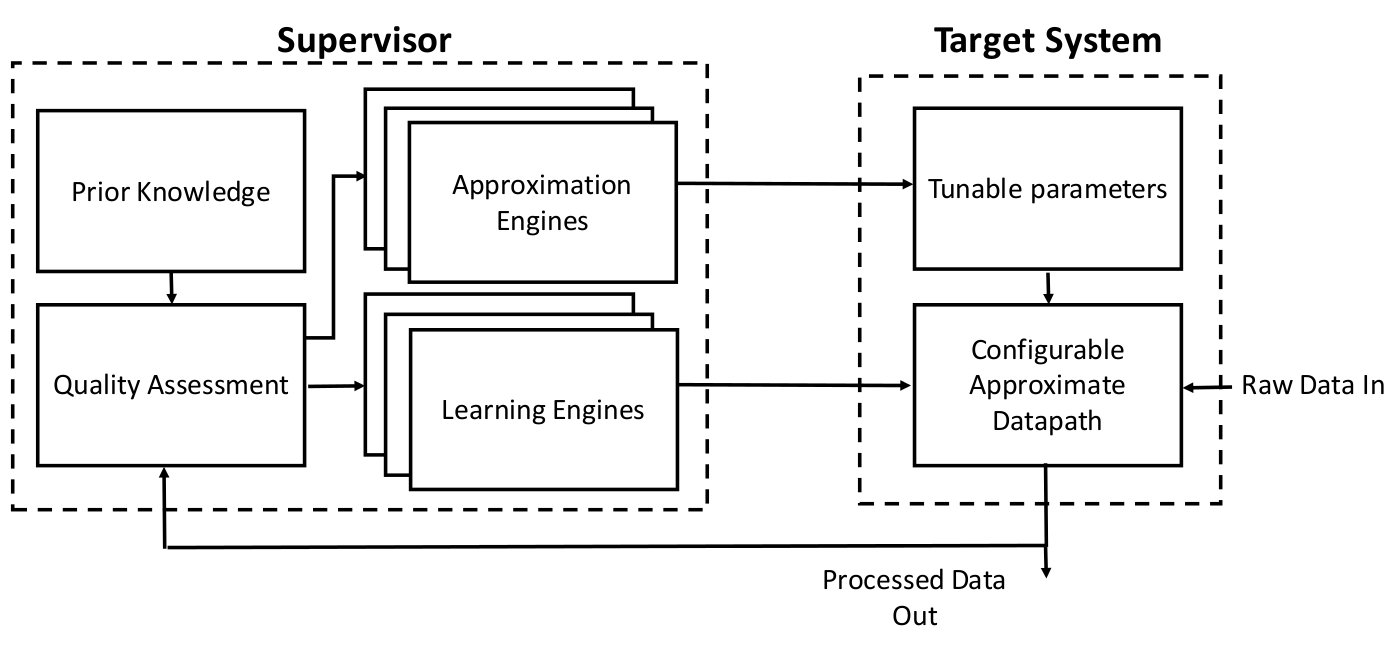
\includegraphics[width=\columnwidth]{img/block_diagram.png}
  \caption{Block diagram}
  \label{fig:block_diagram}
\end{figure}

\section{Approximation methodology}\label{learning}

Our methodology is based on equipping the processing pipeline with variable levels of approximation, i.e., configurable approximations, and an approximation engine within a supervisor block (which may contain additional optimisations such as parameter tuning): a block diagram is depicted in Fig. \ref{fig:block_diagram}. Depending on the application and the deployment technology (e.g., CPU, ASIC, FPGA) the nature of approximations varies, but our method is applicable across the entire spectrum. Traditional approximation methods include bit width reduction \cite{mittal2016survey}, memoisation \cite{sinha2016low}, predictive memory access \cite{yazdanbakhsh2016mitigating}, arithmetic re-writes \cite{nepal2016automated}, input-based approximations \cite{raha2016input}, etc.
\par Based on prior knowledge about the data, our approximation engine dynamically monitors the processing pipeline's output, and verifies whether or not the calculations still obey the assumptions about the data. If yes, then it is assumed that current levels of accuracy are still within error bounds: hence, the pipeline can be approximated further. If not, then it is assumed that accuracy has exceeded error bounds, and the level of approximation is reduced. Using this method, it is possible to converge on an approximation strategy that optimises power consumption \textit{in situ}, without access to ground truth. 

\par Our approach is predicated on runtime-configurable levels of approximation. In software solutions running on CPUs and GPUs, this can be achieved through different software versions \cite{vassiliadis2015programming} or through Instruction Set Architecture (ISA) level approximations \cite{Vassiliadis:2015:PMR:2858788.2688546}. In bespoke hardware solutions implemented on ASIC or FPGA, through configurable hardware versions which clock- or power-gate accurate circuitry; this is the approach we use on our experiments, which we detail in Section \ref{experiments}.

%\begin{figure}[tb]
%  \centering
%  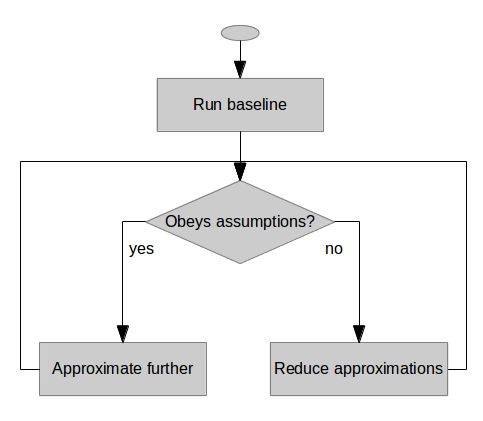
\includegraphics[width=0.7\columnwidth]{img/flowchart.png}
%  \caption{Approximation engine's runtime behaviour.}
%  \label{fig:flowchart}
%\end{figure}

\section{Case study: EKF tracking}
\label{sec:EKF}
The proposed approximate computing algorithm is evaluated for a non-linear, Gaussian, single-target tracking problem. It is assumed that the target is circularly rotating over the $xy$-plane. To have the paper self-contained and to simplify explaining the points at which approximation is imposed, the motion model and EKF equations are detailed in this section.

It is assumed that the sensor measures the range and bearing (azimuth) of the target in meters and radians, respectively. This is a typical sensing scenario in LiDAR, radar and stereo vision used in numerous applications, e.g., autonomous vehicles \cite{7398055},

\begin{equation}
\left\{
\begin{array}{l}
r_k = \sqrt{\bar{x}_k^2 + \bar{y}_k^2} + n_{r_k} \\
\phi_k = atan2(\bar{y}_k, \bar{x}_k) + n_{\phi_k}
\end{array}
\right.,
\label{eq:Meas}
\end{equation}

\noindent where $\bar{x}_k$ and $\bar{y}_k$ are the true states of the target location, ${\bf Z}_k = [r_k, \phi_k]$ contains the measured range and bearing values, and ${\bf N}_k = [n_{r_k}, n_{\phi_k}]$ is a random vector sampled from a Gaussian with zero mean, and all are at the $k^{th}$ iteration. $atan2(.)$ computes the angle between the point (vector) $[\bar{x}_k, \bar{y}_k]$ and positive $x$-axis.

\begin{figure}[tb]
  \centering
  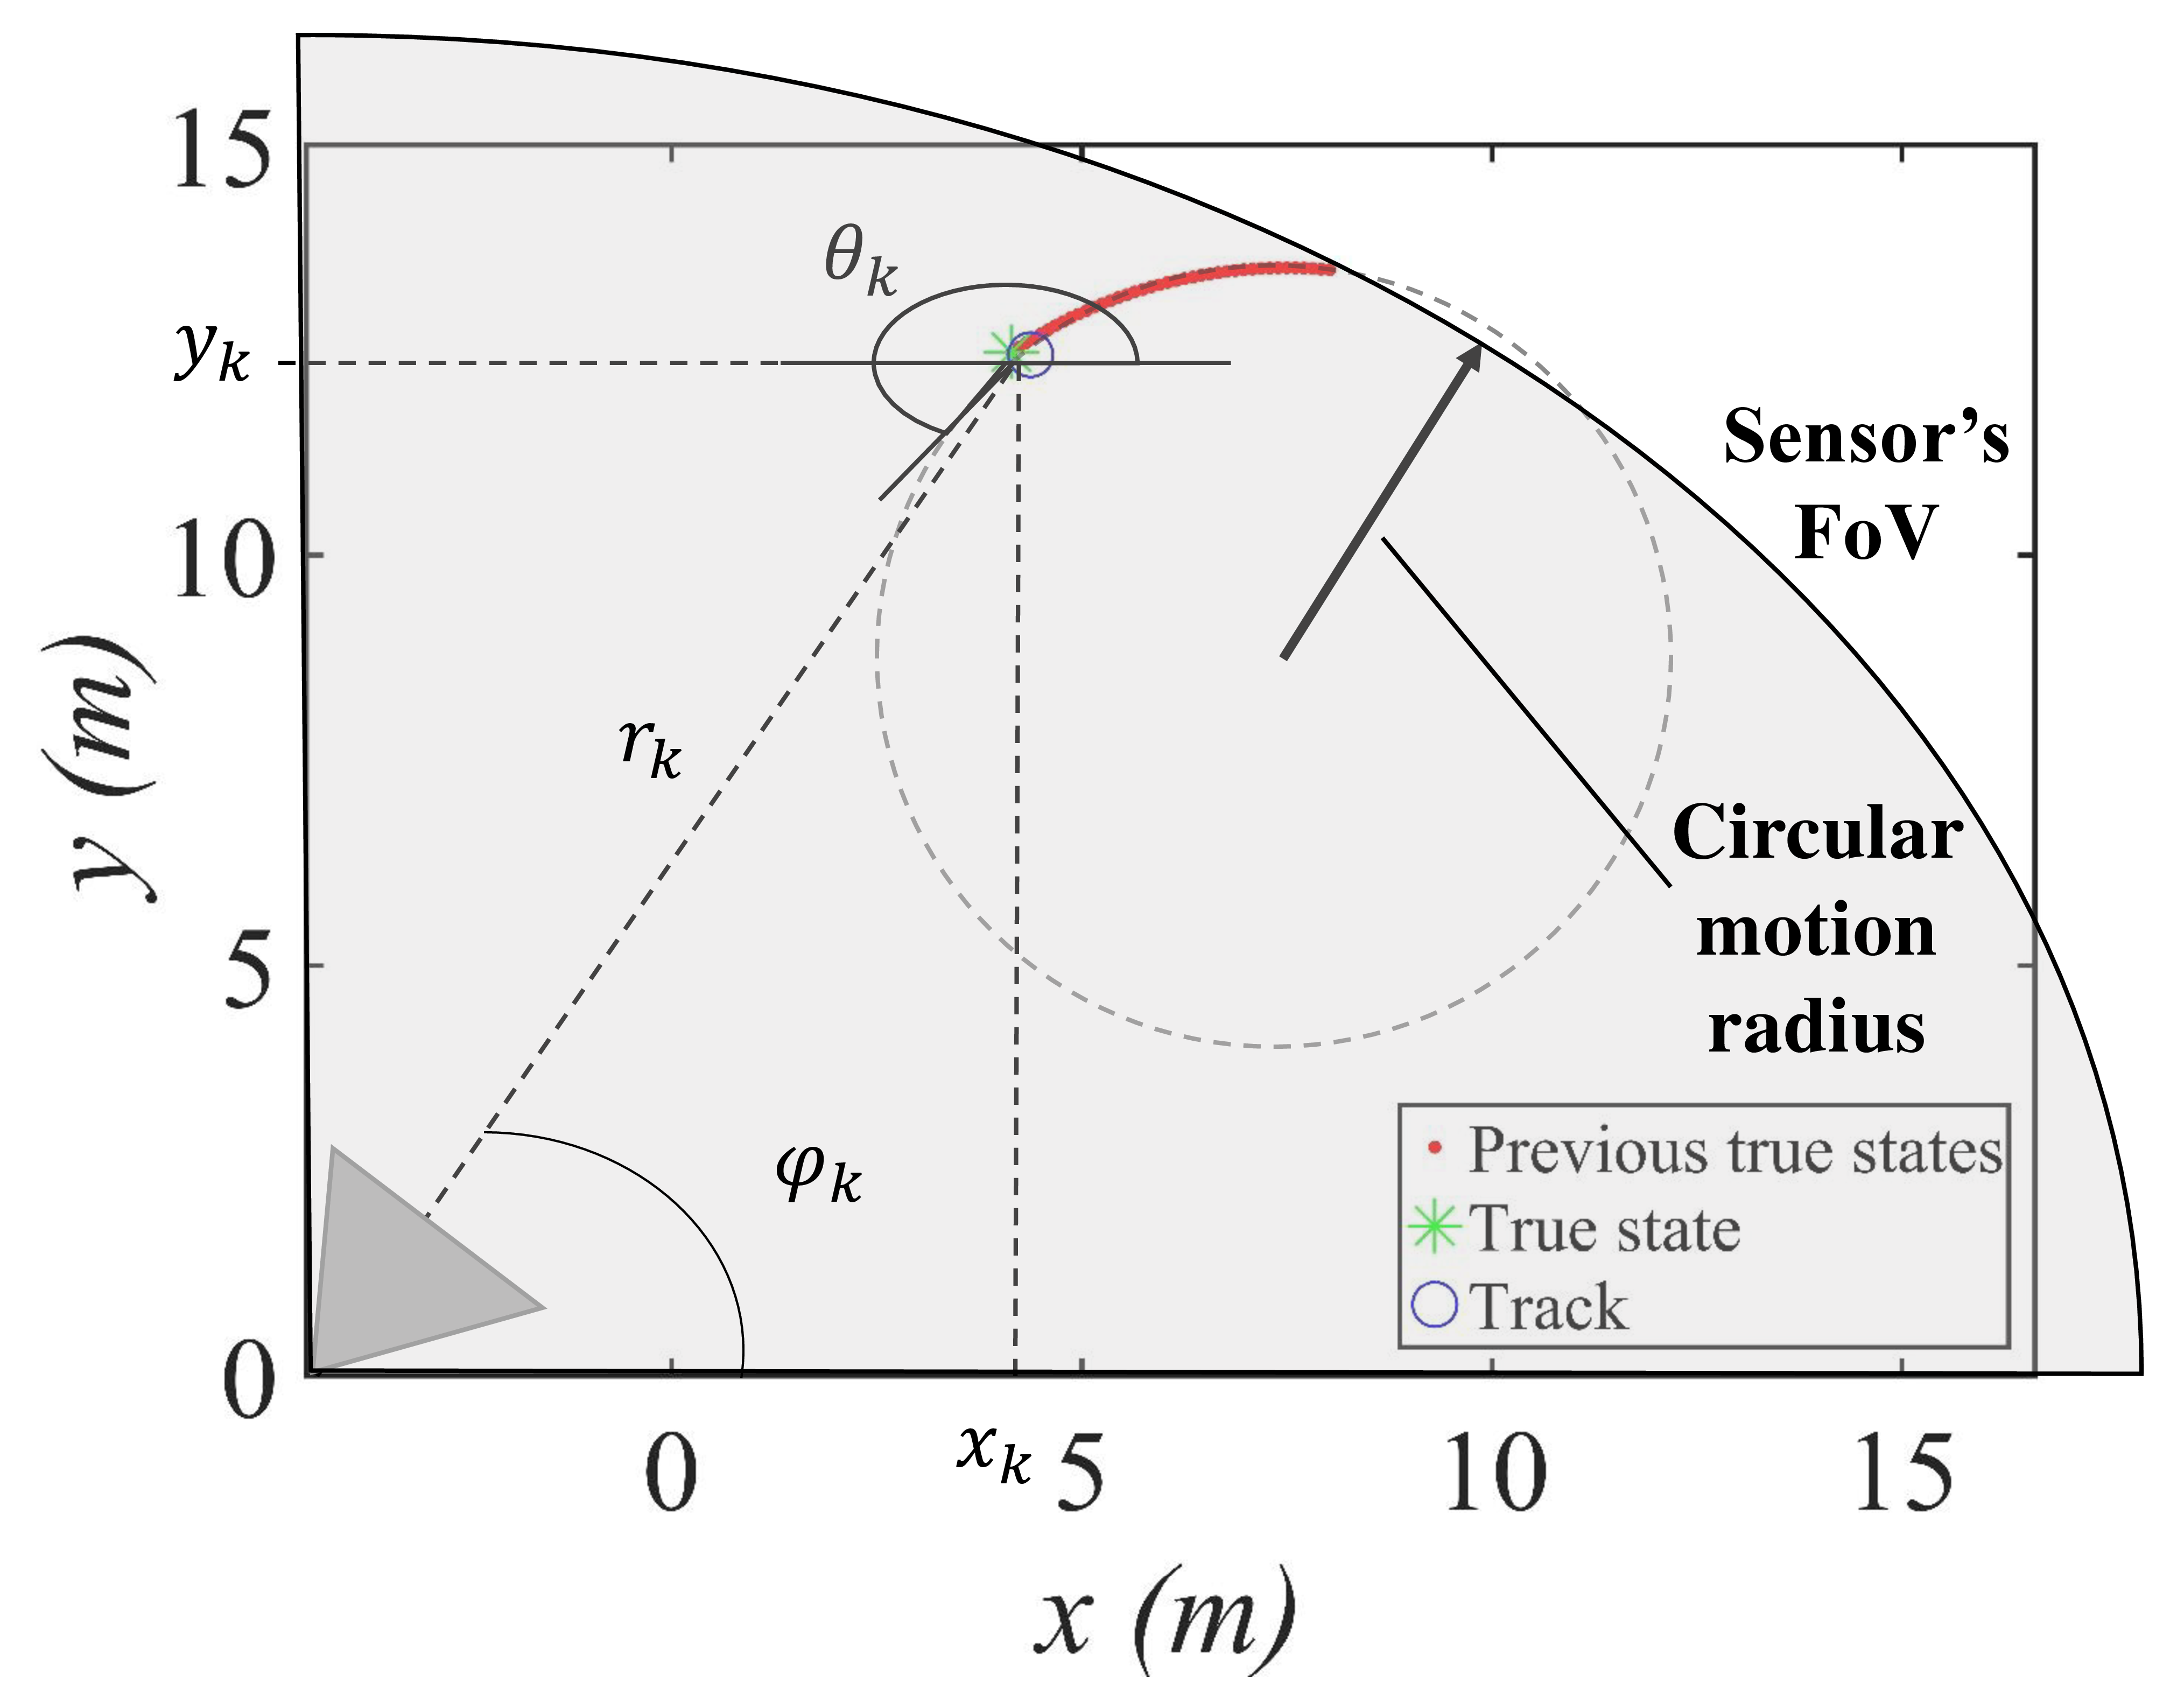
\includegraphics[width=0.95\columnwidth]{img/Trackingfinal.png}
  \caption{The tracking scene containing the FoV of the sensor, target motion trajectory and state parameters definition.}
  \label{fig:TrackScene}
\end{figure}

It is assumed that at time $k$, the target has a three dimensional state vector ${\bf X}_k = [x_k, y_k, \theta_k]^\intercal$, in which $[x_k, y_k]$ and $\theta_k$ are the position and pose states of the target, respectively. This is shown in Fig.~\ref{fig:TrackScene}. The state estimation equations are,

\begin{equation}
\left\{
\begin{array}{l}
\hat{x}_k = x_{k-1} + (\Delta t) v_k \cos(w_k \Delta t + \theta_{k-1}) + m_{x_k} \\
\hat{y}_k = y_{k-1} + (\Delta t) v_k \sin(w_k \Delta t + \theta_{k-1}) + m_{y_k} \\
\hat{\theta}_k = \theta_{k-1} + w_k \Delta t + m_{\theta_k}
\end{array}
\right..
\label{eq:State}
\end{equation}

\noindent ${\bf u}_k = [v_k, w_k]$ is the speed vector containing the radial and angular speed parameters in m$/$sec and rad$/$sec, respectively, which can be computed from previous state vectors. $\Delta t$ is the time update resolution in seconds. $\hat{{\bf X}}_k = [\hat{x}_k, \hat{y}_k, \hat{\theta}_k]^\intercal$ is the estimated state vector for the $k^{th}$ iteration. ${\bf M}_k = [m_{x_k}, m_{y_k}, m_{\theta_k}]^\intercal$ is a random vector sampled from a Gaussian distribution with zero mean. 

Due to the non-linearity in (\ref{eq:Meas}) and (\ref{eq:State}), Gaussianity will not be preserved and therefore, a linear approximation is used based on Taylor series expansion. 
The Jacobian matrix for the estimation step is computed using \ref{eq:State} as follows:

\begin{equation}
{\bf J}_{X, k-1} = \left[
\begin{array}{llr}
1 & 0 & -(\Delta t) v_k \sin(w_k \Delta t + \theta_{k-1}) \\
0 & 1 &  (\Delta t) v_k \cos(w_k \Delta t + \theta_{k-1}) \\
0 & 0 & 1 
\end{array}
 \right].
\end{equation}

\noindent Assuming ${\bf \Sigma}_{{X}, k-1}$ and ${\bf Q}_{k}$ are the state and noise covariance matrices at $k-1$ and $k$, the estimated state covariance matrix at iteration $k$ will be: ${\bf \Sigma}_{\hat{X}, k} = {\bf J}_{X, k-1}{\bf \Sigma}_{X, k-1}{\bf J}_{X, k-1}^\intercal + {\bf Q}_{k}$.

The correction step of EKF incorporates the measurement at time $k$. Let ${\bf R}_k$ be the measurement covariance matrix. Then the corrected state vector can be computed as follows,

\begin{equation}
\begin{array}{l}
{\bf X}_{k} = \hat{{\bf X}}_k + {\bf K}_k ({\bf Z}_k - h(\hat{{\bf X}}_k)) \\
{\bf K}_k = {\bf \Sigma}_{\hat{X}, k} {\bf H}_k^\intercal {\bf S}_k^{-1} \\
{\bf S}_k = {\bf H}_k {\bf \Sigma}_{\hat{X}, k} {\bf H}_k^\intercal + {\bf R}_k
\end{array}.
\end{equation}

\noindent ${\bf K}_k$ is the Kalman gain, ${\bf S}_k$ is the innovation covariance and ${\bf X}_{k}$ is the (corrected) state vector at the $k^{th}$ iteration. $h(.)$ is a non-linear function, which maps the current estimated target state to the coordinate frame of the sensor. ${\bf H}_k$ is the measurement's Jacobian matrix, which is computed as follows using \ref{eq:Meas},

\begin{equation} 
{\bf H}_k = 
\frac{1}{\sqrt{x_k^2 + y_k^2}}
\left[
\begin{array}{lll}
x_k & y_k & 0 \\
-y_k & x_k & 0
\end{array}
\right].
\end{equation}

\noindent The corrected covariance matrix for the $k^{th}$ iteration will then be,

\begin{equation}
{\bf \Sigma}_{X, k} = 
\left(
\left[
\begin{array}{lll}
1 & 0 & 0 \\ 
0 & 1 & 0 \\
0 & 0 & 1 
\end{array}
\right]
- {\bf K}_k {\bf H}_k
\right)
{\bf \Sigma}_{\hat{X}, k}.
\label{eq:correctCOV}
\end{equation}

\subsection{KL divergence for Gaussian motion}
Comparison with the prior knowledge can be performed in various ways. 
For an iterative filtering, which estimates and corrects the state of the object using the obtained measurements, the prior knowledge can be defined using the target's motion. Any deviation from this known model can be used to compromise over approximation during run-time. 

One solution to quantify such model is to stack state vectors for a given number of consecutive iterations. Then estimating the statistics of the stacked tracks, using either parametric or non-parametric approaches, can be used to map the result to our prior knowledge. 

To be more specific, in this paper, we use a parametric approach to approximate the probability density function (PDF) of the stacked target states from iteration $k$ to $k+N$, i.e. ${\bf s}_{k:k+N}$. 
Our prior knowledge is then compared with the computed approximated PDF. In our work, we use KL divergence to perform this task as follows,

\begin{equation}
D_{KL}({\bf H}_{k, N} || {\bf H}_{p}) = \sum_{i}{{\bf H}_{k, N}} \log{\frac{{\bf H}_{k, N}}{{\bf H}_{p}}}
\label{eq:KLDIV1}
\end{equation}

\noindent in which ${\bf H}_{k, N}$ is the approximated PDF of the $k^{th}$ to $(k+N)^{th}$ state samples and ${\bf H}_{p}$ is the "prior knowledge" PDF of the target's motion.

For this experimental setting, we assume that the object's motion statistics remains Gaussian (our prior knowledge). This can be iteratively evaluated by (\ref{eq:KLDIV1}). It can be easily shown that the KL divergence for two Gaussian distributions can be simplified as follows,

\begin{equation}
D_{KL}({\bf H}_{k, N} || {\bf H}_{p}) = \log{\frac{\sigma_p}{\sigma_{k, N}}} + \frac{\sigma_{k, N}^2 + (\mu_{k, N} - \mu_p)^2}{2\sigma_p^2} - \frac{1}{2}
\label{eq:KLDIV2}
\end{equation}

\noindent in which, ($\mu_{k, N}$, $\sigma_{k, N}^2$) and ($\mu_p$, $\sigma_p^2$) are the mean vector and variance of the stacked samples and prior knowledge, respectively. For our experiments, we assume that $\mu_p$ is the radius of the target's circular rotation, which is known with a $\pm \sigma_p$ standard deviation (both in meters).

We define the stacked samples ${\bf s}_{k:k+N}$ as the Euclidean distance between the target state $[x_k, y_k]^\intercal$ and centre of rotation.
The mean and variance $\mu_{k, N}$ and $\sigma_{k, N}^2$ are then computed as follows,

\begin{equation}
\begin{array}{l}
\mu_{k, N} = \frac{\sum_{i}{{s}^i_{k:k+N}}}{N} \\
\sigma_{k, N}^2 = \frac{\sum_{i}{({s}^i_{k:k+N}} - \mu_{k, N})^2}{N}
\end{array}
\end{equation}

\noindent in which, ${s}^i_{k:k+N}$ is the $i^{th}$ element in ${\bf s}_{k:k+N}$. Small values for $D_{KL}(.)$ correspond to higher similarity between the prior knowledge and tracks. Therefore, more intense approximation is imposed. On the other hand, the approximation level is reduced once the $D_{KL}(.)$ is higher than a given threshold.

\section{Experimental results}\label{experiments}

Fig. \ref{fig:experimental_flow} presents our methodology to obtain accuracy and power profiles for several degrees of approximation, and to generate a version with configurable approximations. 
\par We begin by implementing EKF in Matlab in applying several algorithm-specific approximations (described in detail in Sub-Section \ref{subsec:profiles}). Matlab simulations are performed to obtain accuracy profiles for each approximation at this step. Matlab Coder is then used to generate C code corresponding to the exact and various approximated versions. C code generated by Matlab is not directly synthesizable to FPGA: hence, we refactor it manually to obtain synthesizable versions. Functionality and corresponding accuracy are not affected by this step. We then apply algorithm-independent approximations on this refactored C code, and use a High Level Synthesis tool (Xilinx Vivado HLS) to generate Verilog Hardware Description Language (Verilog HDL) exact and approximated versions. Matlab's HDL coder offers a direct route from Matlab to FPGA, but not all language constructs are supported and it would not enable to us to perform algorithm-independent optimisations: hence the use of HLS through Xilinx's tools.
\par RTL simulation and FPGA synthesis (we target Virtex 7 technology) is performed through Xilinx Vivado Design Suite to obtain resource usage and power consumption. Power consumption is estimated through Xilinx Power Estimator tool embedded in Vivado, which uses resource usage information and switching rates obtained from RTL simulation to calculate a high accuracy measure of power consumption. This step enables us to obtain power profiles for each approximation.
\par The final step combines the various versions into one configurable solution. This is an FPGA implementation which combines accurate and approximated versions, where the level of approximations can be configured and modified at runtime. Unused logic (e.g., an exact version of some operation when running in corresponding approximate mode) is clock gated to eliminate dynamic power consumption. This version is then used to obtain results for dynamic approximations by the approximation engine using prior knowledge.  


\subsection{Power and Accuracy Profiles}\label{subsec:profiles}

Algorithm-dependent approximations are modifications on the implementation of certain constructs, which vary from algorithm to algorithm. These can be complete re-writes of algorithm functionality; however, since our goal is to determine the validity of prior knowledge for runtime approximations, simple arithmetic re-writes suffice. We implemented four different re-writes:

\begin{enumerate}
\item COS re-write: cosine functions are replaced by quantized look-up tables. The HDL implementation of cosines is realized through a look-up table, but by re-writing at Matlab level, we can control the level of quantization: the approximated version is more quantized (i.e., requires fewer data) than the default Vivado HLS implementation.
\item SIN re-write: identically to cosine, sine functions are re-written using a quantized loop-up table.
\item SQRT re-write: the square root of the sum of squares $\sqrt{x^2+y^2}$, which requires two DSP multipliers and a look-up table for the square root, is replaced by a sum of absolutes $\left| x\right|+\left| y\right|$, which requires only two conversions to unsigned and an adder.
\item ATAN re-write: the arc tangent function, realized by default through a look up table, is approximated through the first three terms of a Taylor series, requiring only arithmetic operations.
\end{enumerate}

\par We detailed several algorithm-independent approximations in Section \ref{learning}. In our experiments, we implemented bit width reduction, from floating to fixed point. The default bit width is 64 bits (Matlab generates double precision floating point operations). Our approximations replaces 64 bits data with fixed point 27 bits data (15 integer and 12 fractional bits). This is one of the fixed point bit widths recommended for power reductions in the Virtex 7 family. 

\begin{table}[h]
\begin{tabular}{r c c c c}
\toprule
Version & \multicolumn{3}{c}{Power (W)} & \% of baseline\\
 & Static & Dynamic & Total &\\
\hline
Exact & 0.247 & 0.552 & 0.799 & 100\%\\
COS & 0.247 & 0.523 & 0.770 & 96.37\%\\
SIN & 0.247 & 0.523 & 0.770 & 96.37\%\\
SQRT & 0.247 & 0.534 & 0.781 & 97.74\%\\
ATAN & 0.247 & 0.532 & 0.779 & 97.49\%\\
27 bits Fixed Point & 0.246 & 0.538 & 0.785 & 98.24\%\\
\hline
\end{tabular}
\caption{Power profiles for exact and each individual approximation.}
\label{table:power_profiles}
\end{table}


\par We ensured that during our RTL simulations, 100 iterations of the complete function are performed, using the same randomly generated input data for all versions, in order to obtain representative activity that ensures high confidence in the power estimation. Table \ref{table:power_profiles} depicts power consumption for the exact and each individual approximated version. Static power remains constant across approximations because the contribution of on-chip memories (BRAMs) dominates, and the number remains constant except for a small reduction when reducing bit widths. 
\par Our next set of experiments started measuring the power consumption of versions that combine bit width reduction with several of the other approximations: results are presented in Table \ref{table:power_profiles_comb}.



\begin{table}[h]
\begin{tabular}{r c c}
\toprule
Approximations (using 27FP) & Power (W) & \% of baseline\\
\hline
COS & 						0.756	& 94.61\%\\
SIN & 						0.756	& 94.61\%\\
SQRT & 						0.767	& 95.99\%\\
ATAN & 						0.765	& 95.74\%\\
COS \& SIN & 				0.741	& 92.74\%\\
COS \& SQRT& 				0.767	& 95.99\%\\
COS \& ATAN & 				0.736	& 92.11\%\\
SIN \& SQRT & 				0.738	& 92.36\%\\
SIN \& ATAN & 				0.736	& 92.11\%\\
SQRT \& ATAN & 				0.747	& 93.49\%\\
COS \& SIN \& SQRT & 		0.709	& 88.73\%\\
COS \& SIN \& ATAN& 		0.707	& 88.48\%\\
COS \& SQRT \& ATAN& 		0.718	& 89.86\%\\
SIN \& SQRT \& ATAN  & 		0.718	& 89.86\%\\
COS \& SIN \& SQRT \& ATAN &0.689 	& 86.23\%\\
\hline
\end{tabular}
\caption{Power profiles for combinations of different approximations.}
\label{table:power_profiles_comb}
\end{table}


\par We use Matlab simulation to determine the accuracy of each combination, compared to the baseline. Table \ref{table:acc_profiles} depicts the accuracy of each version. Results in the "Absolute" tab are the mean and standard deviation ($\sigma$), respectively, of the absolute error (in meters) compared to the ground truth (real object position) in our simulation. Results in the "Accuracy" tab are the ratios, for mean and standard deviation, between the exact version results and the absolute value of the difference between exact and approximate results.
    


\begin{table}[h]
\begin{tabular}{r c c c c}
\toprule
Version & \multicolumn{2}{c}{Absolute (m)} & \multicolumn{2}{c}{Accuracy (\%)}\\
 & Mean & $\sigma$ & Mean & $\sigma$\\
\hline
Exact	& 0.5633 & 0.3092 & 100 & 100\\
\hline
COS & 						0.6742	& 0.2805	& 83.55 & 89.76 \\
SIN & 						0.6524	& 0.3652	& 86.34 & 84.66 \\
SQRT & 						0.6968	& 0.3764	& 80.84 & 82.14 \\
ATAN & 						3.3520	& 1.7953	& 16.80 & 17.22 \\
COS \& SIN & 				0.6044	& 0.3973	& 93.19 & 77.82 \\
COS \& SQRT& 				0.7497	& 0.4101	& 75.13 & 75.39 \\
COS \& ATAN & 				0.9771	& 0.6937	& 57.65 & 44.57 \\
SIN \& SQRT & 				0.7353	& 0.3711	& 76.60 & 83.31 \\
SIN \& ATAN & 				7.7667	& 2.5248	& 7.252 & 12.24 \\
SQRT \& ATAN & 				1.4812	& 0.8149	& 38.02 & 37.94 \\
COS \& SIN \& SQRT & 		0.5870	& 0.3680	& 95.96 & 84.02 \\
COS \& SIN \& ATAN& 		1.7503	& 1.0135	& 32.18 & 30.50 \\
COS \& SQRT \& ATAN& 		0.9949	& 0.7006	& 56.61 & 44.13 \\
SIN \& SQRT \& ATAN  & 		7.7528	& 2.5424	& 7.265 & 12.16 \\
COS \& SIN \& SQRT \& ATAN &1.8295 	& 1.0765	& 30.78 & 28.72 \\
\hline
\end{tabular}
\caption{Accuracy profiles for combinations of different approximations. Exact version uses double floating point precision (64 bits); every other version uses 27 bits fied point precision.}
\label{table:acc_profiles}
\end{table}

\par The final integrated version with configurable approximations, including clock gated logic, is compared against the baseline in Table \ref{table:integrated}.

\begin{table}[h]
\begin{tabular}{r c c c c c c c}
\toprule
 & \multicolumn{3}{c}{Power (W)} & \multicolumn{4}{c}{FPGA Resources}\\
 & Static & Dynamic & Total & LUT & FF & DSP & BRAM\\
\hline
Exact & 0.247 & 0.552 & 0.799 & 46449 & 17666 & 61 & 55\\
Approx. & 0.246 & 0.443 & 0.689 & 44995 & 16981 & 58 & 55\\
\hline
\end{tabular}
\caption{Resource usage and ower consumption for baseline and final configurable approximations version.}
\label{table:integrated}
\end{table}








\subsection{Dynamic approximations using prior knowledge}

\begin{figure}[tb]
  \centering
  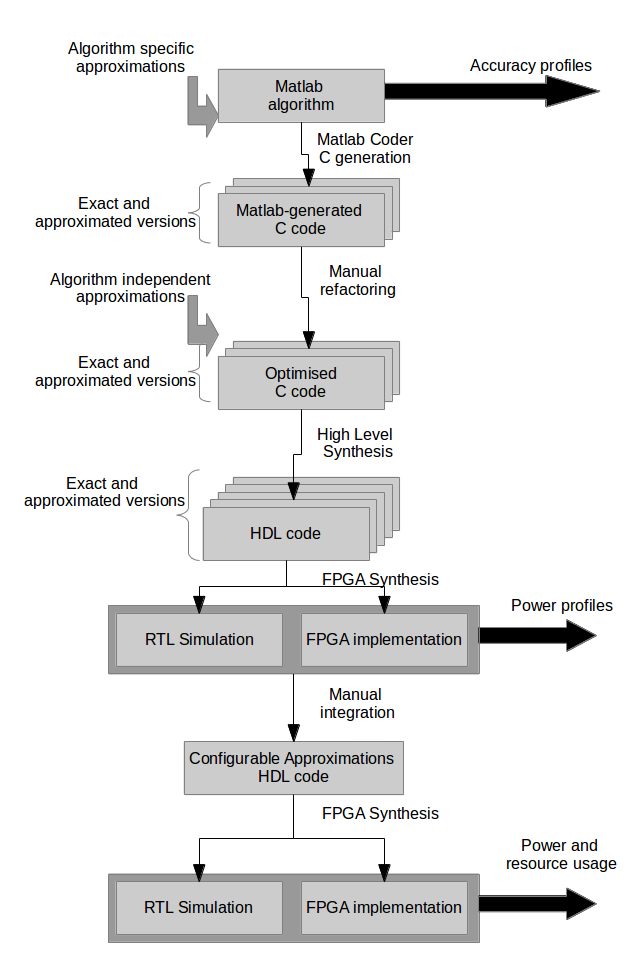
\includegraphics[width=0.9\columnwidth]{img/experimental_flow.png}
  \caption{Experimental design flow.}
  \label{fig:experimental_flow}
\end{figure}

\section{Conclusions and future work}\label{conclusions}
We have described the use of prior knowledge to perform runtime approximations, without access to ground truth. Our experiments, on a tracking application using EKF, demonstrate that prior knowledge can indeed be used to ensure that accuracy is within acceptable bounds, without having to perform empirical evaluations based on representative test data. Our results support the conclusion that approximate computing need not be limited to design time: thus enabling power optimisations with the same degree of runtime configuration as traditional performance optimisations.
\par Future work will address three limitations of our study: (a) the approximation engine, which leverages prior knowledge, is external to the test system: hence, its power contribution was not modeled. We will integrate a hardware version embedded in the processing pipeline so power evaluation is completely accurate. (b) the utilized approximations are \textit{ad hoc} heuristics, and result in a poor theoretical lower limit to power consumption (86.23\%). We will adopt more sophisticated approximation methodologies, using state of the art automated tools and benchmarks, in order to obtain greater power savings. (c) We have only modeled one case study; we will experiment with several different algorithms from various domains in order to evaluate the coverage of our approach, in function of different types of application-specific prior knowledge.


%\par This paper presents two main contributions:

%\begin{itemize}
%\item We describe a method for cross-stage analysis which enables novel approximations, compared to the state of the art. Our method re-organizes and flattens the separation of processing pipelines in order to identify approximation opportunities which are not transformed by traditional local methods.
%\item We investigate the possibility of approximations on control flow, rather than just data processing. This is achieved through high-level information, i.e., task-level, which is made available to approximate control flow instructions
%\item We describe a method for runtime approximations. By analysing and exploiting dynamic features, i.e., information which is only available at runtime (input dependent), our method dynamically approximates processing, achieving power reductions through optimizations which would have been deemed too accuracy-impacting at design time. We evaluate our approach on an approximate ISA processor.
%\end{itemize}





%\section{Control-Flow Approximations}

%\begin{itemize}
%\item why control flow cannot easily be approximated
%\item show dataflow-style code structure
%\item show applications which fit that structure
%\item introduce concept of probabilistic branching
%\item show probabilistic branching for runtime approximations
%\item compare with software code modification
%\end{itemize}



% The very first letter is a 2 line initial drop letter followed
% by the rest of the first word in caps.
% 
% form to use if the first word consists of a single letter:
% \IEEEPARstart{A}{demo} file is ....
% 
% form to use if you need the single drop letter followed by
% normal text (unknown if ever used by the IEEE):
% \IEEEPARstart{A}{}demo file is ....
% 
% Some journals put the first two words in caps:
% \IEEEPARstart{T}{his demo} file is ....
% 
% Here we have the typical use of a "T" for an initial drop letter
% and "HIS" in caps to complete the first word.



% needed in second column of first page if using \IEEEpubid
%\IEEEpubidadjcol




% An example of a floating figure using the graphicx package.
% Note that \label must occur AFTER (or within) \caption.
% For figures, \caption should occur after the \includegraphics.
% Note that IEEEtran v1.7 and later has special internal code that
% is designed to preserve the operation of \label within \caption
% even when the captionsoff option is in effect. However, because
% of issues like this, it may be the safest practice to put all your
% \label just after \caption rather than within \caption{}.
%
% Reminder: the "draftcls" or "draftclsnofoot", not "draft", class
% option should be used if it is desired that the figures are to be
% displayed while in draft mode.
%
%\begin{figure}[!t]
%\centering
%\includegraphics[width=2.5in]{myfigure}
% where an .eps filename suffix will be assumed under latex, 
% and a .pdf suffix will be assumed for pdflatex; or what has been declared
% via \DeclareGraphicsExtensions.
%\caption{Simulation results for the network.}
%\label{fig_sim}
%\end{figure}

% Note that the IEEE typically puts floats only at the top, even when this
% results in a large percentage of a column being occupied by floats.


% An example of a double column floating figure using two subfigures.
% (The subfig.sty package must be loaded for this to work.)
% The subfigure \label commands are set within each subfloat command,
% and the \label for the overall figure must come after \caption.
% \hfil is used as a separator to get equal spacing.
% Watch out that the combined width of all the subfigures on a 
% line do not exceed the text width or a line break will occur.
%
%\begin{figure*}[!t]
%\centering
%\subfloat[Case I]{\includegraphics[width=2.5in]{box}%
%\label{fig_first_case}}
%\hfil
%\subfloat[Case II]{\includegraphics[width=2.5in]{box}%
%\label{fig_second_case}}
%\caption{Simulation results for the network.}
%\label{fig_sim}
%\end{figure*}
%
% Note that often IEEE papers with subfigures do not employ subfigure
% captions (using the optional argument to \subfloat[]), but instead will
% reference/describe all of them (a), (b), etc., within the main caption.
% Be aware that for subfig.sty to generate the (a), (b), etc., subfigure
% labels, the optional argument to \subfloat must be present. If a
% subcaption is not desired, just leave its contents blank,
% e.g., \subfloat[].


% An example of a floating table. Note that, for IEEE style tables, the
% \caption command should come BEFORE the table and, given that table
% captions serve much like titles, are usually capitalized except for words
% such as a, an, and, as, at, but, by, for, in, nor, of, on, or, the, to
% and up, which are usually not capitalized unless they are the first or
% last word of the caption. Table text will default to \footnotesize as
% the IEEE normally uses this smaller font for tables.
% The \label must come after \caption as always.
%
%\begin{table}[!t]
%% increase table row spacing, adjust to taste
%\renewcommand{\arraystretch}{1.3}
% if using array.sty, it might be a good idea to tweak the value of
% \extrarowheight as needed to properly center the text within the cells
%\caption{An Example of a Table}
%\label{table_example}
%\centering
%% Some packages, such as MDW tools, offer better commands for making tables
%% than the plain LaTeX2e tabular which is used here.
%\begin{tabular}{|c||c|}
%\hline
%One & Two\\
%\hline
%Three & Four\\
%\hline
%\end{tabular}
%\end{table}


% Note that the IEEE does not put floats in the very first column
% - or typically anywhere on the first page for that matter. Also,
% in-text middle ("here") positioning is typically not used, but it
% is allowed and encouraged for Computer Society conferences (but
% not Computer Society journals). Most IEEE journals/conferences use
% top floats exclusively. 
% Note that, LaTeX2e, unlike IEEE journals/conferences, places
% footnotes above bottom floats. This can be corrected via the
% \fnbelowfloat command of the stfloats package.








% if have a single appendix:
%\appendix[Proof of the Zonklar Equations]
% or
%\appendix  % for no appendix heading
% do not use \section anymore after \appendix, only \section*
% is possibly needed

% use appendices with more than one appendix
% then use \section to start each appendix
% you must declare a \section before using any
% \subsection or using \label (\appendices by itself
% starts a section numbered zero.)
%





% use section* for acknowledgment
\section*{Acknowledgment}
We acknowledge the support of the Engineering and Physical Research
Council, grant references EP/K009931/1 (Programmable embedded
platforms for remote and compute intensive image processing
applications), EP/K014277/1 (MOD University Defence Research Collaboration in Signal Processing) and EP/N012402/1 (TASCC: Pervasive low-TeraHz and Video Sensing for Car Autonomy and Driver Assistance (PATH CAD)).



% Can use something like this to put references on a page
% by themselves when using endfloat and the captionsoff option.
\ifCLASSOPTIONcaptionsoff
  \newpage
\fi



% trigger a \newpage just before the given reference
% number - used to balance the columns on the last page
% adjust value as needed - may need to be readjusted if
% the document is modified later
%\IEEEtriggeratref{8}
% The "triggered" command can be changed if desired:
%\IEEEtriggercmd{\enlargethispage{-5in}}

% references section

% can use a bibliography generated by BibTeX as a .bbl file
% BibTeX documentation can be easily obtained at:
% http://mirror.ctan.org/biblio/bibtex/contrib/doc/
% The IEEEtran BibTeX style support page is at:
% http://www.michaelshell.org/tex/ieeetran/bibtex/
%\bibliographystyle{IEEEtran}
% argument is your BibTeX string definitions and bibliography database(s)
%\bibliography{IEEEabrv,../bib/paper}
%
% <OR> manually copy in the resultant .bbl file
% set second argument of \begin to the number of references
% (used to reserve space for the reference number labels box)
\bibliographystyle{IEEEtran}
\bibliography{references}

% biography section
% 
% If you have an EPS/PDF photo (graphicx package needed) extra braces are
% needed around the contents of the optional argument to biography to prevent
% the LaTeX parser from getting confused when it sees the complicated
% \includegraphics command within an optional argument. (You could create
% your own custom macro containing the \includegraphics command to make things
% simpler here.)
%\begin{IEEEbiography}[{\includegraphics[width=1in,height=1.25in,clip,keepaspectratio]{mshell}}]{Michael Shell}
% or if you just want to reserve a space for a photo:

%\begin{IEEEbiography}{Michael Shell}
%Biography text here.
%\end{IEEEbiography}

% if you will not have a photo at all:
%\begin{IEEEbiographynophoto}{John Doe}
%Biography text here.
%\end{IEEEbiographynophoto}

% insert where needed to balance the two columns on the last page with
% biographies
%\newpage

%\begin{IEEEbiographynophoto}{Jane Doe}
%Biography text here.
%\end{IEEEbiographynophoto}

% You can push biographies down or up by placing
% a \vfill before or after them. The appropriate
% use of \vfill depends on what kind of text is
% on the last page and whether or not the columns
% are being equalized.

%\vfill

% Can be used to pull up biographies so that the bottom of the last one
% is flush with the other column.
%\enlargethispage{-5in}



% that's all folks
\end{document}


